\chapter{Statistical Analysis of Time Series Data}

\noindent Pandas makes it simple to perform statistical analysis on dataframes, which is extremely important in determining different indicators and acting as inputs to the learning algorithms.\\

\section{Global statistics}
\noindent For example, if you had a dataframe $df1$ which had the closing prices for various stocks over a given time period, you can retrieve an ndarray with the mean of the columns by just calling $df1.mean()$.

\begin{figure}[h]
\begin{lstlisting}[style=python]
SPY     126.396777
IBM     166.380238
GLD     145.029775
AAPL    399.498435
XOM      77.054682
dtype: float64
\end{lstlisting}
\caption{Example output array for $mean()$ (called on closing prices for January 2010 through December 2012)}
\end{figure}

\noindent In addition to $mean$, there around 32 other global statistics that are available in pandas.

\section{Rolling statistics}

\noindent Instead of doing analysis on the entire dataset, you might want to do a rolling analysis, which only looks at certain snapshots of the data to sample. For example, you could have a 20-day moving mean, which you would calculate day-by-day by averaging the last 20 days' data. In later sections, this moving average will be explained in more detail, but some critical points of interest are when the moving average crosses the data.

\subsection{Bollinger bands\textsuperscript{\textregistered}}

\noindent Some analysts believe that significant deviations from the moving mean will result in movement back towards the mean. If the price dips far below the mean, then it might be a buy signal, whereas if it goes too high, it could indicate a time to sell. Bollinger bands are a way of measuring this deviation.\\

\noindent Bollinger observed that if you look at the volatility of the stock, and if it's too large, then you discard the movements above and below the mean, but if it's not, then it might be worth paying attention to.\\

\noindent What he did was place two new moving means, one $2\sigma$ above, and another $2\sigma$ below the moving average. If you look at deviations near to $2\sigma$, then they're worth paying attention to. If the price drops \textit{below} $2\sigma$, and then rises back up through it, then it could be a buy signal. (the price is moving back towards the average).\\

\noindent Conversely, if the price rises above $2\sigma$, then falls back down, it could be a sell signal.

\subsection{Computing rolling statistics in pandas}
\noindent Pandas provides some methods to easily calculate rolling mean ($rolling\_mean()$) and rolling standard deviation ($rolling\_std$).\\

\noindent\begin{minipage}{\linewidth}

\noindent\textit{example 11:} Calculating a 20-day rolling mean

\lstinputlisting[style=python,firstline=37,lastline=37]{code_examples/statistics_1.py}
\end{minipage}

\begin{figure}[h!]
	\centering
	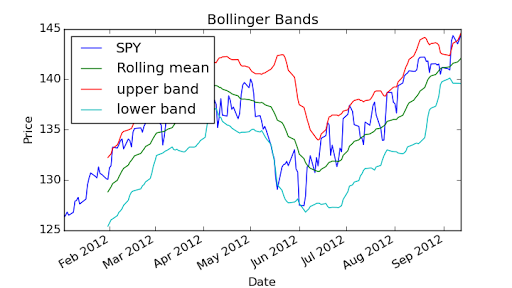
\includegraphics[width=\textwidth]{images/bollinger_bands.png}
    \caption{Plot of rolling mean for \textit{SPY} with Bollinger bands\textsuperscript{\textregistered}}
\end{figure}
\newpage

\noindent The Bollinger bands\textsuperscript{\textregistered} were calculated as follows:\\

\noindent\textit{example 12:} Calculating bollinger bands

\lstinputlisting[style=python]{code_examples/statistics_1.py}

\section{Daily returns}
\noindent Daily returns are how much a stock's price went up or down on a given day. They are an extremely important statistic as they can be a good comparison between different stocks.

\begin{equation*}
	daily\_ret[t] = \frac{price[t]-price[t-1]}{price[t-1]} = \frac{price[t]}{price[t-1]}-1
\end{equation*}

\begin{lstlisting}[style=python]
daily_ret = (df / df.shift(1).values) - 1
daily_ret.ix[0,:] = 0
\end{lstlisting}

\begin{figure}[h!]
	\centering
	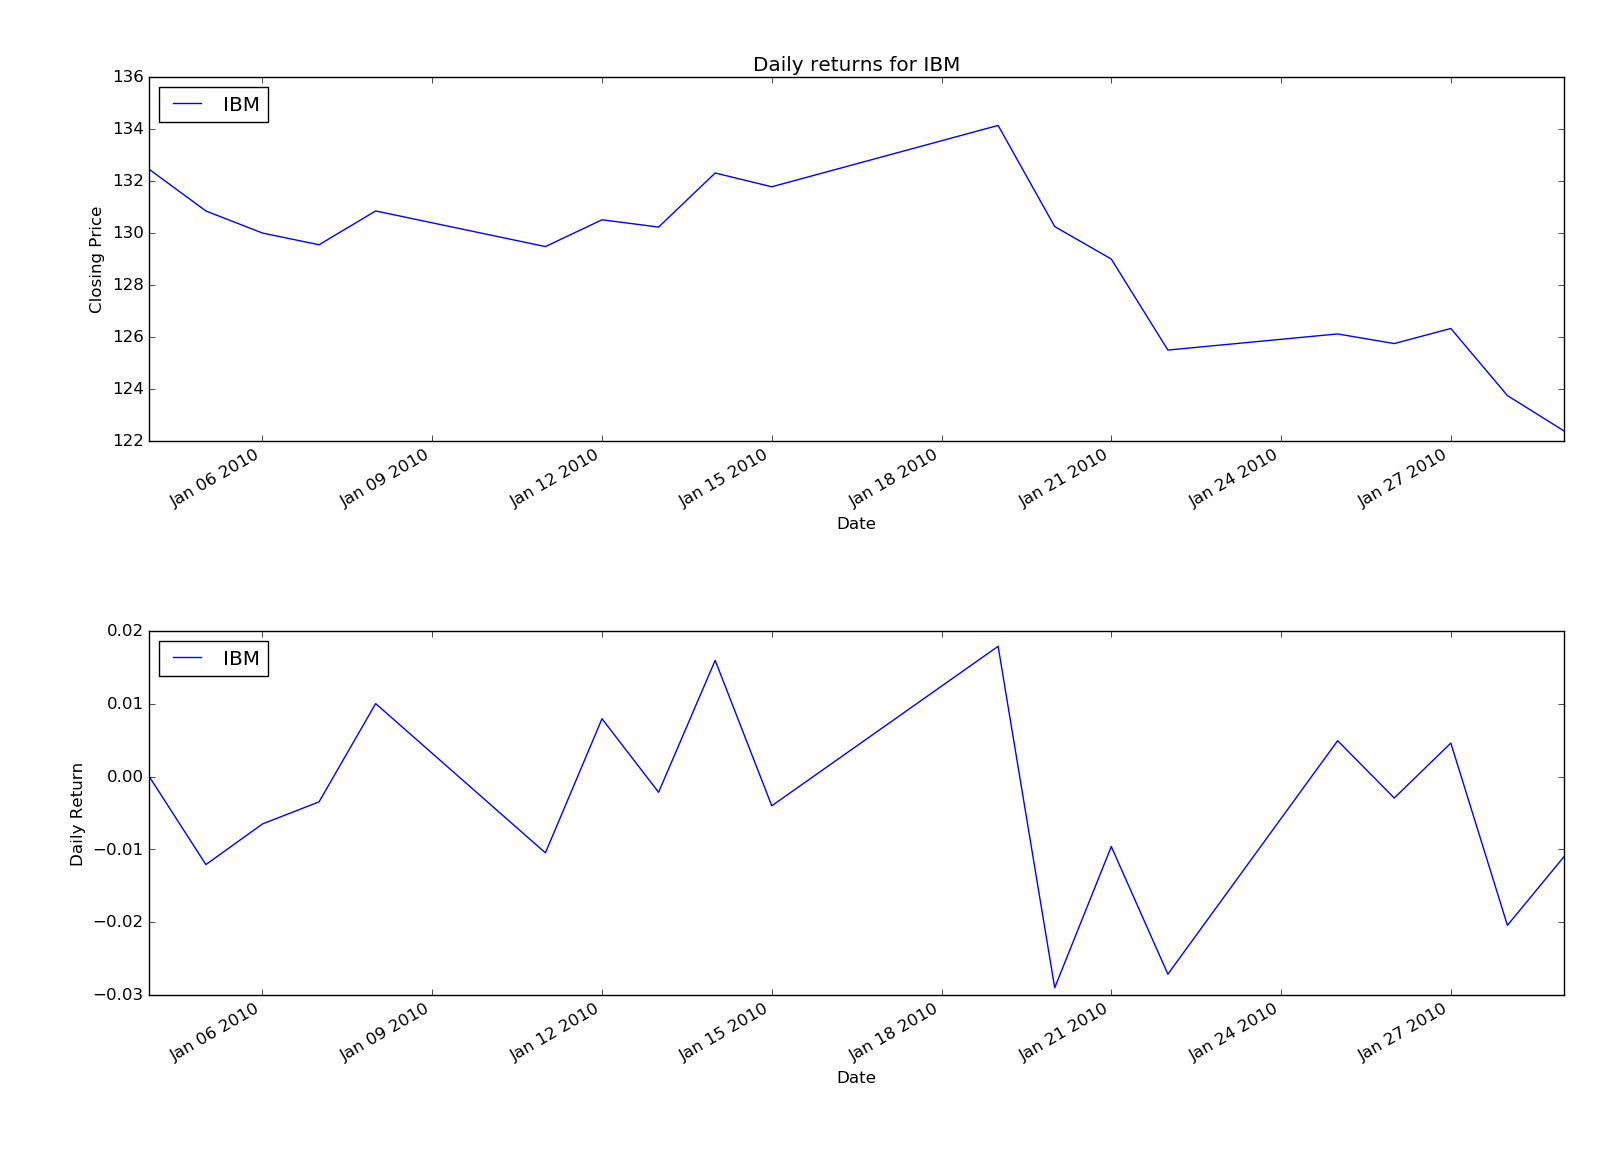
\includegraphics[width=\textwidth]{images/daily_returns.png}
    \caption{Plot of \textit{IBM}'s prices (top) with daily returns (bottom)}
\end{figure}

\section{Cumulative Returns}
\noindent Cumulative return is calculated by finding the gain from the beginning of the range to the current time, i.e.

\begin{equation*}
	cum\_ret[t] = \frac{price[t]}{price[0]}-1
\end{equation*}

\noindent For example, if the price at the beginning was \$125, and the current price is \$142, then the gain/cumulative return is $\frac{142}{125}-1 = .136 (13.6\%)$\\

\noindent Cumulative returns are essentially the original dataset normalized.

\section{Incomplete data}
\noindent People assume that financial data is extremely well-documented and that perfect data is recorded minute by minute. They also believe that there are no gaps or missing data points. However, for any particular stock, it might have different prices on different stock exchanges! It's difficult to know who's right all the time. Also, not all stocks trade every day (they might suddenly start trading or stop trading).\\

\noindent You might think you can just interpolate the data between breaks, but that'd cause statistical errors and a side-effect of "looking into the future" when doing analysis on that subset of data. The better way of doing it to minimize error is to fill forward and backwards.

\subsection{Filling}
\noindent To fix the "NaN"/empty data, you can use filling to maintain the last known value until known data is reached. For example, if you had a stock that didn't have data until 2001 and then stopped having data in 2006 but then started having data again in 2012, you could fill forward from 2006-2012 and then fill backwards from 2001 back to whenever you want your data to start.\\

\noindent\begin{minipage}{\linewidth}

\noindent\textit{example 13:} Filling in missing data using $fillna()$
\begin{lstlisting}[style=python]
df = get_data(symbols,dates)

df.fillna(method="ffill",inplace=True)
df.fillna(method="bfill",inplace=True)
\end{lstlisting}
\end{minipage}

\begin{figure}[h!]
	\centering
	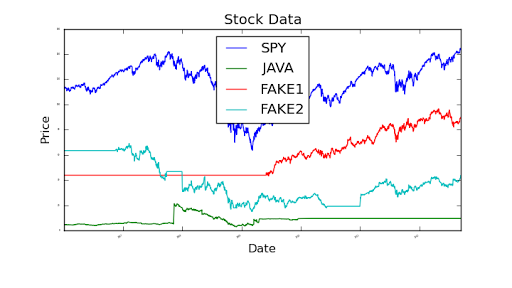
\includegraphics[width=\textwidth]{images/filled_data.png}
    \caption{Data will forward and backwards filled values (horizontal lines)}
\end{figure}
\newpage

\section{Histograms and scatter plots}
\noindent It's difficult to draw conclusions directly from daily returns plots, so histograms make it easier to see what's going on. A histogram allows you to see how many occurrences of each return happens relative to other returns. This histogram typically follows a Gaussian over large periods of time.\\

\subsection{Histograms}

\noindent From the histogram we can determine a few key statistics: mean, standard deviation, and kurtosis. Kurtosis is a measure of how close the curve is to a Gaussian. In stock data, there are usually more occurrences at high deviations (causing sort of "fat tails"), which would be reflected as a positive kurtosis. Skinny tails would mean a negative kurtosis.

\begin{figure}[h!]
	\centering
	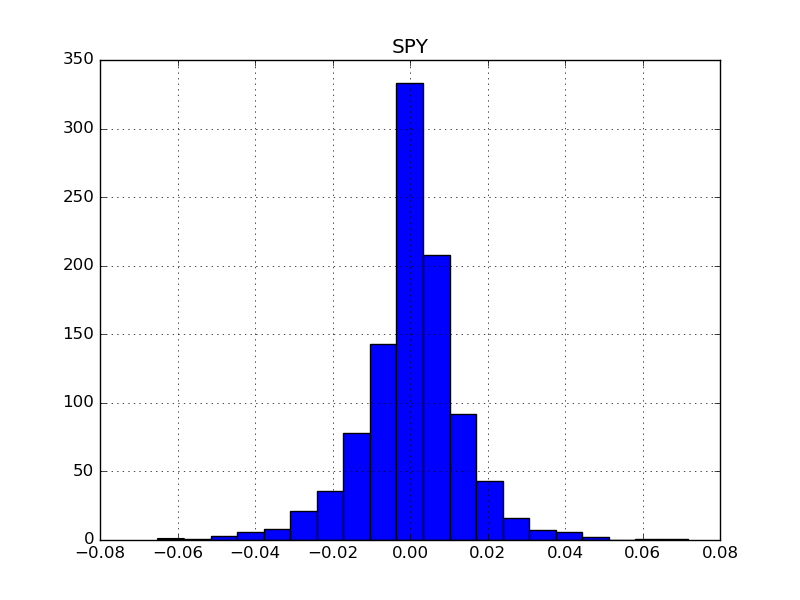
\includegraphics[width=\textwidth]{images/histograms_1.png}
    \caption{Histogram of daily returns \textit{SPY} from January 2009 through December 2012}
\end{figure}
\newpage

\noindent\begin{minipage}{\linewidth}
\noindent\textit{example 14:} Getting a histogram
\noindent The histogram above was generated by just calling $hist()$ on the daily returns dataframe as such:

\begin{lstlisting}[style=python]
daily_returns.hist(bins=20)
\end{lstlisting}
\end{minipage}

\noindent The $bins$ parameter is essentially the resolution of the histogram. The domain is divided into 20 bins and anything within those bins counts for that bin's count in the histogram.

\noindent Other statistics like mean and standard deviation are easily calculated:

\noindent\begin{minipage}{\linewidth}
\begin{lstlisting}[style=python]
mean = daily_returns['SPY'].mean()
print "mean=",mean

std = daily_returns['SPY'].std()
print "std deviation=",std
\end{lstlisting}
\end{minipage}

\noindent\begin{minipage}{\linewidth}
\noindent Which outputs:
\begin{lstlisting}[style=python]
mean= 0.000509326569142
std deviation= 0.0130565407719
\end{lstlisting}
\end{minipage}

\noindent\begin{minipage}{\linewidth}
\noindent We can now plot the mean and standard deviations on the plot to make analysis easier:
\begin{lstlisting}[style=python]
plt.axvline(mean,color='w',linestyle='dashed',linewidth=2)
plt.axvline(mean+std,color='r',linestyle='dashed',linewidth=2)
plt.axvline(mean-std,color='r',linestyle='dashed',linewidth=2)
\end{lstlisting}
\end{minipage}

\begin{figure}[h!]
	\centering
	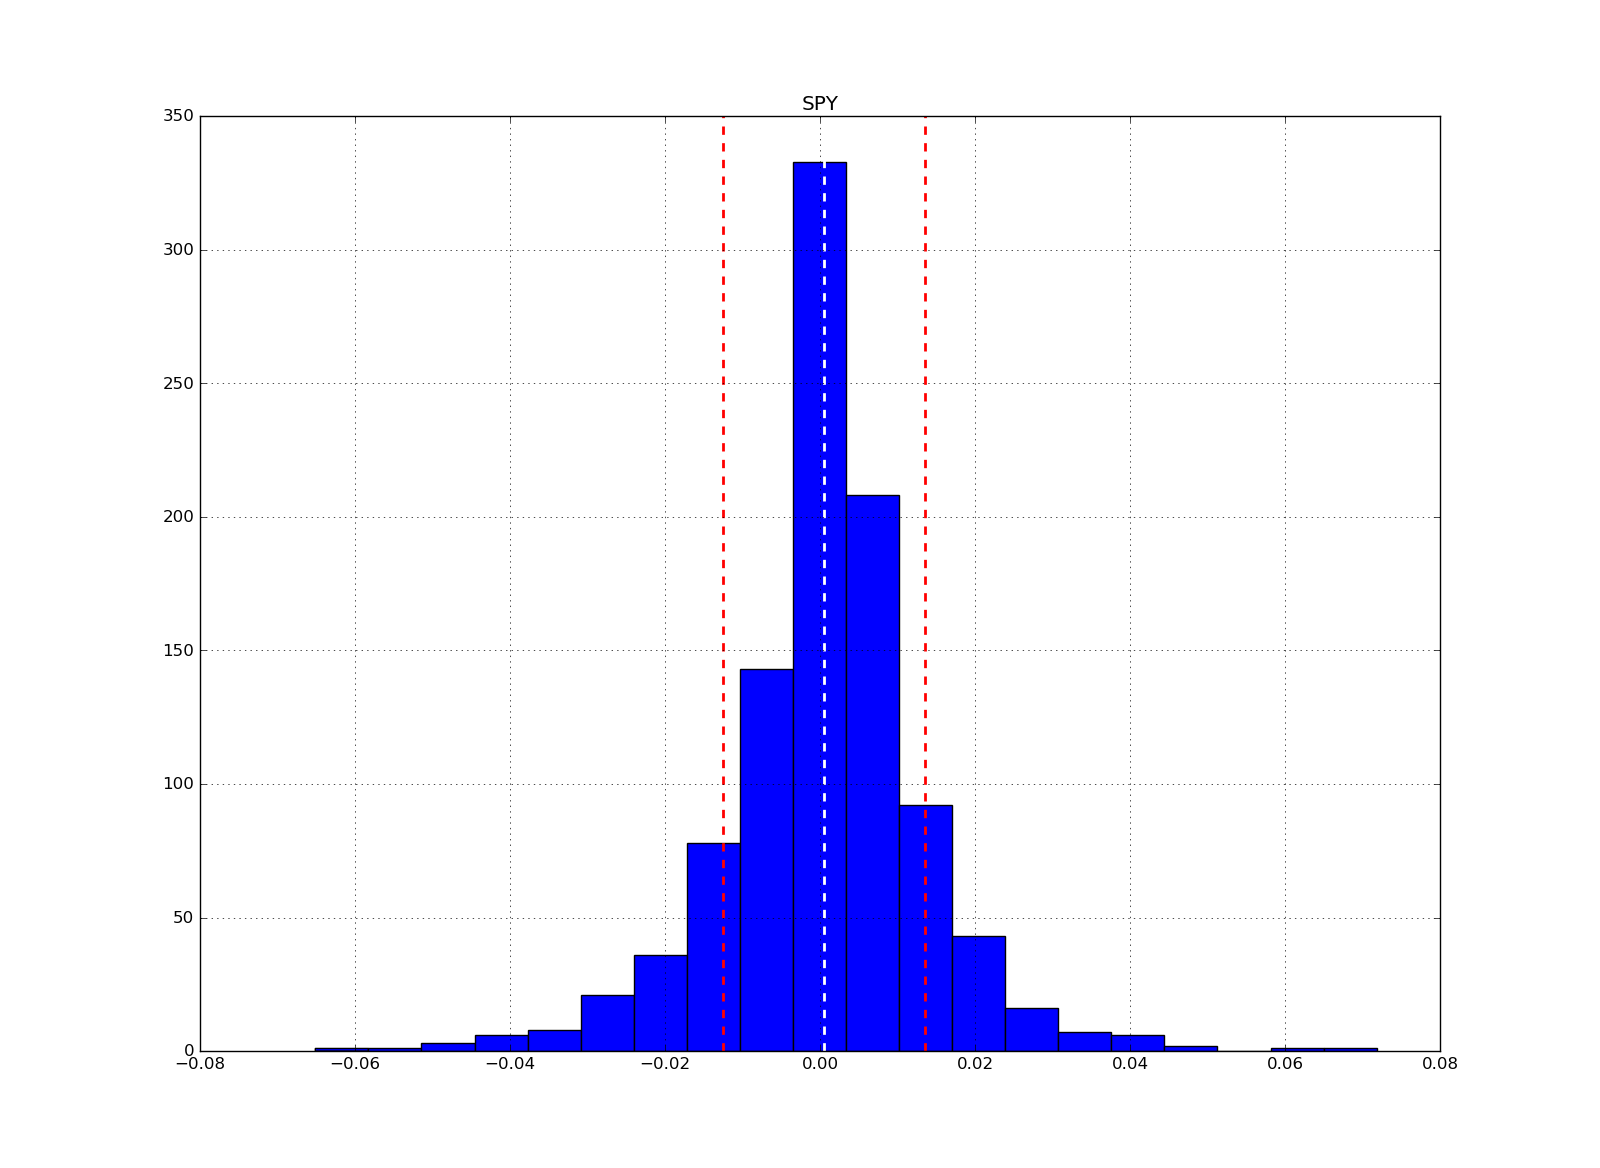
\includegraphics[width=\textwidth]{images/histograms_2.png}
    \caption{Histogram with mean (white) and $1\sigma$ (red) plotted}
\end{figure}

\noindent\begin{minipage}{\linewidth}
\noindent The output of
\begin{lstlisting}[style=python]
print daily_returns.kurtosis()
\end{lstlisting}
\end{minipage}

\noindent\begin{minipage}{\linewidth}
\noindent is:
\begin{lstlisting}[style=python]
SPY    3.376644
\end{lstlisting}
\end{minipage}

\noindent which means that the data has fat tails since it's positive.\\

\noindent The utility of these histograms comes when plotting them together. It's easy to compare multiple stocks in terms of their returns and volatility. If stock A's curve is skewed more positive and is thinner than stock B, then it has a low volatility with higher returns vs stock B.\\

\begin{figure}[h!]
	\centering
	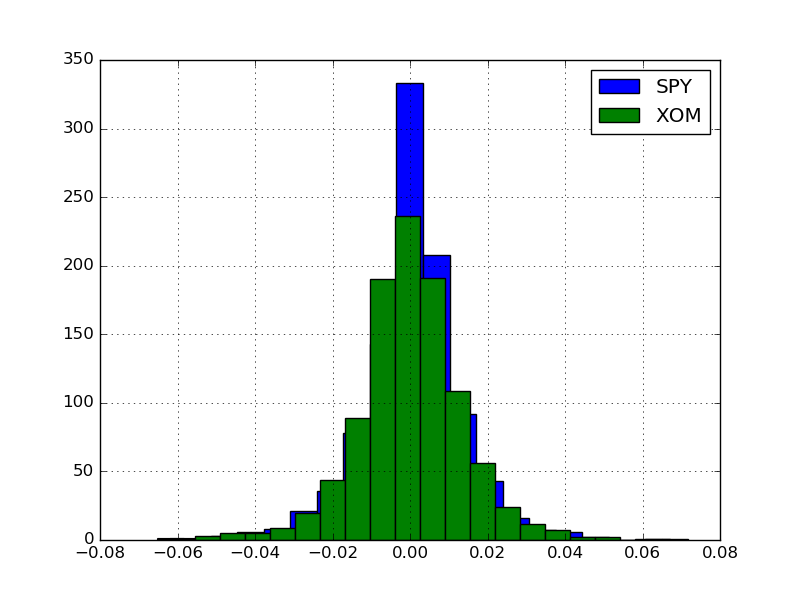
\includegraphics[width=\textwidth]{images/histograms_comparison.png}
    \caption{Histogram comparison of \textit{SPY} and \textit{XOM}}
\end{figure}
\newpage
\noindent By looking at this chart, you can see that \textit{SPY} and \textit{XOM} are about the same in volatility ($\sigma_{SPY} = .013057, \sigma_{XOM} = .013647$). However, \textit{SPY} would have higher returns since $\overline{R_{SPY}} = .000509$ whereas $\overline{R_{XOM}} = .000151$ 

\subsection{Scatter plots}
\noindent Scatter plots are another way of visualizing the correlation between two stocks. Say you had a dataframe with the daily returns for \textit{SPY} and \textit{XYZ}. If you took just the $ndarray$ containing the y-axis values, and then plotted \textit{SPY} on the x-axis and \textit{XYZ} on the y-axis, you would see a bunch of points that might have a certain trend.\\

\noindent If you take a linear regression of this data, the slope would be called the beta ($\beta$) value. If the $\beta$ value for \textit{SPY} and \textit{XYZ} is 1, it means that, on average, if \textit{SPY} (the market) moves up by 1\%, then \textit{XYZ} also moves up by 1\%.\\

\noindent The y-intercept of the line is called $\alpha$. It describes how the stock on the y-axis performs with respect the stock on the x-axis. If the $\alpha$ value of \textit{XYZ} with respect to \textit{SPY} is positive, then, on average, \textit{XYZ} is returning more than the market overall.

\paragraph{Correlation} If there isn't any correlation in the dataset, then the linear regression doesn't tell you anything about the relationship. A common method for calculating the correlation is by finding the \textit{sample Pearson correlation coefficient, $r_{xy}$}. It's calculated by the following:

\begin{equation*}
	r_{xy} = \frac{cov(X,Y)}{\sigma_{X}\sigma_{Y}} = \frac{\sum_{i=1}^{n}(x_i - \bar{x})(y_i - \bar{y})}{\sqrt{\sum_{i=1}^{n}(x_i - \bar{x})^2}\sqrt{\sum_{i=1}^{n}(y_i - \bar{y})^2}}
\end{equation*}

where $cov$ is the covariance. In this case, X would be the daily return for \textit{SPY} and Y would be the daily return for \textit{XYZ}.
\noindent If $|r_{X,Y}| = 1$, then the two are perfectly correlated (either positively or negatively, depending on the sign of $\rho$). If $|r| < 1$, then there is possible correlation, but a value closer to 1 means better correlation. If $r = 0$, there is no correlation. \\

\noindent\begin{minipage}{\linewidth}
\noindent\textit{example 15:} Plotting scatter plots, getting $\alpha$ and $\beta$ values, and determining correlation
\begin{lstlisting}[style=python]
# scatter plot for XOM vs SPY
daily_ret.plot(kind='scatter',x='SPY',y='XOM',title="Scatter plot")
beta_XOM,alpha_XOM = np.polyfit(daily_ret['SPY'],daily_ret['XOM'],1)
plt.plot(daily_ret['SPY'],beta_XOM*daily_ret['SPY']+alpha_XOM,'-',color='r')
plt.show()

# scatter plot for GLD vs SPY
daily_ret.plot(kind='scatter',x='SPY',y='GLD',title="Scatter plot")
beta_GLD,alpha_GLD = np.polyfit(daily_ret['SPY'],daily_ret['GLD'],1)
plt.plot(daily_ret['SPY'],beta_GLD*daily_ret['SPY']+alpha_GLD,'-',color='r')
plt.show()

print "Beta XOM: ", beta_XOM
print "Alpha XOM: ",alpha_XOM
print "Beta GLD: ",beta_GLD
print "Alpha GLD: ",alpha_GLD

# calculate correlation using pearson method
print "Correlation matrix: \n", daily_ret.corr(method='pearson')
\end{lstlisting}
\end{minipage}
\noindent which outputs:
\begin{lstlisting}[style=python]
Beta XOM:  0.85753872112
Alpha XOM:  -0.000285580653638
Beta GLD:  0.0663816850634
Alpha GLD:  0.000660583984316
Correlation matrix: 
          SPY       XOM       GLD
SPY  1.000000  0.820423  0.074771
XOM  0.820423  1.000000  0.079401
GLD  0.074771  0.079401  1.000000
\end{lstlisting}

\noindent Looking at the $\beta$ values, you can see that \textit{XOM} is more responsive to market changes, while \textit{GLD} is relatively unresponsive. However, \textit{GLD} tends to perform better than the market on average, since its $\alpha$ is positive.\\

\noindent But these values are meaningless without seeing what their correlations are. Looking at the correlation matrix, \textit{XOM} is pretty well correlated with \textit{SPY}, whereas \textit{GLD} has a very low correlation, so changes \textit{GLD} aren't really correlated with changes in the market.

\begin{figure}[h!]
	\centering
    \subcaptionbox{\textit{XOM}}[.45\linewidth]{
    	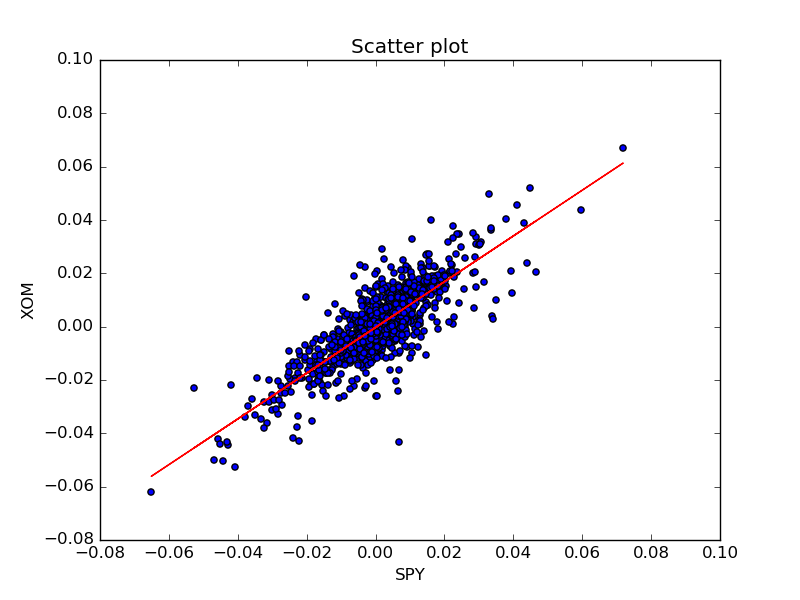
\includegraphics[width=.5\linewidth]{images/scatter_XOM.png}
    }
    \subcaptionbox{\textit{GLD}}[.45\linewidth]{
    	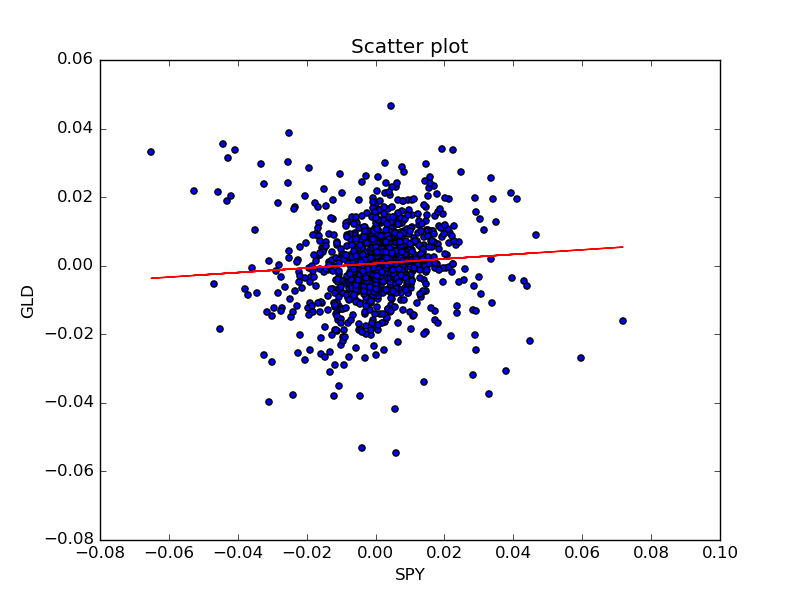
\includegraphics[width=.5\linewidth]{images/scatter_GLD.png}
    }
    \caption{Scatter plots for \textit{XOM} and \textit{GLD}}
\end{figure}
\newpage

\noindent Looking at the plots, it's easy to see that the points for \textit{XOM} are more correlated and match the line better than do those of \textit{GLD}.

\section{Sharpe ratio and other portfolio statistics}

\noindent The \textbf{portfolio} is the collection of all stocks currently owned by a person. It's important to know various statistics associated with the portfolio to make informed decisions on what to sell/buy.

\noindent Suppose you begin with a portfolio $p$ consisting of the following parameters:
\begin{lstlisting}[style=python]
start_val = 1000000
start_date = '2009-01-01'
end_date = '2011-12-31'
symbols = ['SPY','XOM','GOOG','GLD']
allocs = [0.4, 0.4, 0.1, 0.1] # @ beginning, 40% to SPY, 40% to XOM, etc
\end{lstlisting}

\noindent Now suppose we want to find the value of this portfolio day-by-day. If we normalize the portfolio dataframe, we essentially have a dataframe containing cumulative returns for each index. If we multiply this by $allocs$, we get returns scaled by each percentage of the total portfolio. Then, multiply by $start\_val$ to get each stock's total value. Finally, take the sum of this penultimate dataframe to get a single-column dataframe with the total portfolio value at each point in time. In Python,

\noindent\begin{minipage}{\linewidth}
\begin{lstlisting}[style=python]
# get cumulative returns
df = get_data(symbols,pd.date_range(start_date,end_date))
df = normalize(df)

# get changes for each stock by their percentages of the starting value
alloced = df*allocs

# get dollar value of changes
vals = alloced*start_val

# sum to get total value
portfolio_value = vals.sum(axis=1)
\end{lstlisting}
\end{minipage}

\noindent We may now compute various statistics on the portfolio's value.

\paragraph{Daily returns} Obviously, daily returns of the entire portfolio would be an important statistic, as they indicate how the portfolio changes over time. For some statistics, we need to get rid of the 0 at the beginning of the daily return or else it'll throw off the values.

\begin{lstlisting}[style=python]
daily_rets = daily_rets[1:]
\end{lstlisting}

\paragraph{Cumulative returns} The total cumulative return of the portfolio is another interesting statistic, as you can see if the overall gain was positive or negative.
\begin{lstlisting}[style=python]
cum_ret = (port_val[-1]/port_val.ix[0,:]) - 1
\end{lstlisting}

\paragraph{Avg. and Std. Deviation} These two are the main statistics that get thrown off by the 0 at the beginning. If it were there, the mean would be closer to 0, even though technically 0 isn't actually one of the returns.

\begin{lstlisting}[style=python]
avg_daily_ret = daily_rets.mean()
std_daily_ret = daily_rest.std()
\end{lstlisting}

\subsection{Sharpe Ratio}
\noindent The \textbf{Sharpe Ratio} is a metric that adjusts return for risk. It enables a quantitative way to compare two stocks in terms of their returns and volatility. The Sharpe Ratio is calculated based on the assumption that, \textit{Ceteris paribus}\footnote{all else held equal},
\begin{itemize}
	\item Lower risk is better
    \item Higher return is better
\end{itemize}
Being an economic indicator, it also takes into account the opportunity cost/return of putting the money in a risk-free asset such as a bank account with interest.

\noindent A sort of risk-adjusted return may be calculated as follows:
\begin{equation*}
	R_{adj} = \frac{R_p - R_f}{\sigma_p}
\end{equation*}
where $R_p$ is the portfolio return, $R_f$ is the risk-free rate of return, and $\sigma_p$ is the volatility of the portfolio return.

\noindent This ratio is a sort of basis for how the Sharpe Ratio is calculated. The Sharpe Ratio is as follows:

\begin{equation*}
	S = \frac{E[R_p - R_f]}{std(R_p-R_f)}
\end{equation*}

\noindent Since we're looking at past data, the expected value is actually the mean of the dataset, so this becomes:\\

\begin{equation*}
	S = \frac{\overline{(R_p - R_f)}}{std(R_p-R_f)}
\end{equation*}

\noindent One question is where $R_f$ comes from. There are three main ways of getting the data for the risk-free rate:
\begin{enumerate}
	\item The London Inter-Bank Offer Rate (LIBOR)
	\item The interest rate on the 3-month Treasury bill
    \item 0\% (what people have been using recently...)
\end{enumerate}

\noindent LIBOR changes each day, and the Treasury bill changes slightly each day, but interest in bank accounts are typically paid in 6-month or yearly intervals. Using this simple trick, you can convert the annual/biannual amount to a daily amount:\\

\noindent Suppose the yearly interest rate is $I$. If we start at the beginning of the year with a value $P$, the new value after interest is paid will be $P'$. To find the equivalent daily interest value, $I_{eq}$,

\begin{align*}
	P' &= P(1+I_{eq})^{252}\\
    P(1+I) &= P(1+I_{eq})^{252}\\
    1+I &= (1+I_{eq})^{252}\\
    (1+I_{eq}) &= \sqrt[\leftroot{-2}\uproot{2}252]{1+I}\\
    I_{eq} &= \sqrt[\leftroot{-2}\uproot{2}252]{1+I} - 1
\end{align*}

\noindent Therefore, $R_f$, the daily risk-free rate, is just $\sqrt[\leftroot{-2}\uproot{2}252]{1+I} - 1$. The reason it's 252 instead of 365 is because there are only 252 trading days in a year.\\

\noindent Since we're treating $R_f$ as constant, the standard deviation in the denominator just becomes $std(R_p)$, so the final equation for the Sharpe Ratio becomes:

\begin{equation*}
	S = \frac{\overline{(R_p - R_f)}}{\sigma_{R_p}}
\end{equation*}

\paragraph{Sampling rate} The Sharpe Ratio can vary widely depending on the sampling frequency. Since SR is an annual measure, any calculations that are done with samples more frequent than yearly need to be scaled to get the annual ratio. To adjust the calculated Sharpe Ratio to be "annualized", you just multiply by a factor of $\sqrt{\# samples\ per\ year}$. So if you sample daily, the Sharpe Ratio would become:

\begin{equation*}
	S = \frac{\overline{(R_p - R_f)}}{\sigma_{R_p}}\sqrt{252}
\end{equation*}

\noindent\textit{example:} Given 60 days of data with the following statistics:\\
\noindent$R_p = 10 bps$\\
$R_f = 2 bps$\\
$\sigma_{R_p} = 10 bps$,\\
what is the Sharpe Ratio? One $bps$ is one hundredth of a percent.

\begin{equation*}
	S = \frac{\overline{(R_p - R_f)}}{\sigma_{R_p}} = \frac{10-2}{10}\sqrt{252} 
    \approx 12.70
\end{equation*}

\section{Optimizers}
\noindent An optimizer can:
\begin{itemize}
  \item Find minimum/maximum values of functions
  \item Build parameterized models based on data
  \item Refine allocations to stocks in portfolios
\end{itemize}

\noindent For example, say you have the function $f(x) = (x-1.5)^2 + .5$, and you want to find the minimum. It's trivial to use calculus and find the minimum analytically, but you can't always do so if you don't have an analytical model of the data. Let's put this in Python:

\noindent\begin{minipage}{\linewidth}
\begin{lstlisting}[style=python]
import pandas as pd
import matplotlib.pyplot as plt
import numpy as np
import scipy.optimize as spo

def f(x):
	y = (x-1.5)**2 + .5
	print "x = {}, y = {}".format(x,y)
	return y
    
def test_run():
 	guess = 2.0
	min_result = spo.minimize(f, guess, method='SLSQP', options={'disp':True})
	print "minima found at:"
	print "x = {}, y = {}".format(min_result.x,min_result.fun)
    
if __name__ == "__main__":
	test_run()
\end{lstlisting}
\end{minipage}

\noindent\begin{minipage}{\linewidth}
\noindent outputs:
\begin{lstlisting}[style=python]
x = [ 2.], y = [ 0.75]
x = [ 2.], y = [ 0.75]
x = [ 2.00000001], y = [ 0.75000001]
x = [ 0.99999999], y = [ 0.75000001]
x = [ 1.5], y = [ 0.5]
x = [ 1.5], y = [ 0.5]
x = [ 1.50000001], y = [ 0.5]
Optimization terminated successfully.    (Exit mode 0)
            Current function value: [ 0.5]
            Iterations: 2
            Function evaluations: 7
            Gradient evaluations: 2
minima found at:
x = [ 1.5], y = [ 0.5]
\end{lstlisting}
\end{minipage}

\begin{figure}[h!]
	\centering
	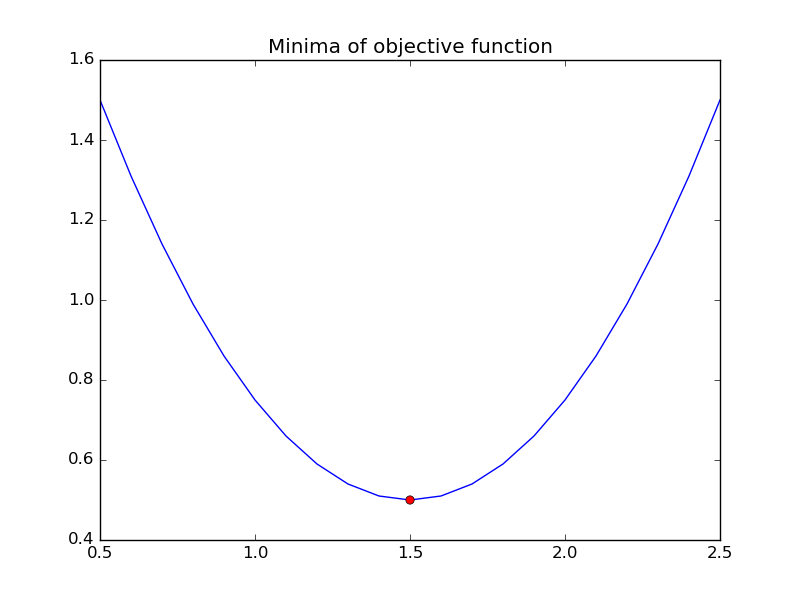
\includegraphics[width=\linewidth]{images/minima.png}
    \caption{Numerical solution to finding the minimum of $f(x) = (x-1.5)^2 + .5$}
\end{figure}
\newpage

\subsection{Pitfalls}
\noindent Optimizers aren't perfect, and since the method used above uses the gradient of the current point to move to the next point, it can be tripped up by various abnormalities in the function it's trying to minimize, such as:

\begin{itemize}
\item\textit{Flat ranges:} If a portion of the graph is flat (the slope is close to or is 0), then the solver will either take a lot of iterations to solve for the minimum or it might not ever be able to move to a new point, unless it can find a way out.
\item\textit{Discontinuities:} If there are discontinuities, the gradient might not be defined well enough for the solver to continue.
\item\textit{Multiple minima:} Say you have a function $f(x) = x^4-2x^2+x^2$. This function has 2 minima at $(0,0)\ and\ (1,0)$. If the solver starts at $x=1.5$, it'll find the minimum at $(1,0)$, but it won't ever reach the other minimum. Conversely, if the solver starts at $x=-1.5$, it'll find the minimum at $(0,0)$. Therefore, it's easy to get trapped in a local minimum that may not be the actual \textit{global} minimum.
\end{itemize}

\subsection{Convex problems}
\noindent A real-valued function $f(x)$ defined on an interval is called \textbf{convex} if the line segment between any two points on the graph of $f(x)$ on that interval lies above the graph. Otherwise, it's called \textbf{non-convex}.

\subsection{Building a parameterized model}
\noindent If you have a set of data points representing rainfall and humidity that were gathered, you might want to find a function that best fits those points. Say you wanted to fit a line $f(x) = mx + b$ to the points. In this case, you can use linear algebra and find the least-squares solution, but you can also use an optimizer to find the \textit{best} parameters $m$ and $b$.\\

\noindent What does "best" mean? Well, we can devise a measure for the error for each point:

\begin{equation*}
	e_i = (y_i - f(x_i))^2 = (y_i - (mx_i+b))^2
\end{equation*}

\noindent which is just the difference between the actual value and our model's predicted value. The reason it's squared is to ensure that negative errors don't reduce the total error when we sum up every $e_i$. 
\begin{equation*}
	E = \sum^{n}_{i=1}(y_i - (mx_i+b))^2
\end{equation*}
\noindent Now that we have what we want to minimize, $E$, we can use a minimizer to find the best $m$ and $b$. To make the parameters nicer to work with in Python (and allow generalization to higher degrees of polynomials), we'll rename $m$ and $b$ to $C_0$ and $C_1$. Now, $f(x) = C_ox+C_1$.

\noindent\begin{minipage}{\linewidth}
\noindent\textit{example 16:}
\begin{lstlisting}[style=python]
import pandas as pandas
import matplotlib.pyplot as plt
import numpy as np
import scipy.optimize as spo

# line is a tuple (C0, C1)
def error(line, data):
	return np.sum((data[:,1] - (line[0]*data[:,0] + line[1])) ** 2)

def fit_line(data,error_func):
	# initial guess for parameters
	l = np.float32([0, np.mean(data[:,1])])

	return spo.minimize(error_func, l, args=(data,), method='SLSQP', options={'disp':True}).x

def test_run():
	original = np.float32([4,2])
	print "original line: C0 = {}, C1 = {}".format(original[0],original[1])
	Xoriginal = np.linspace(0,10,40)
	Yoriginal = original[0]*Xoriginal + original[1]

	plt.plot(Xoriginal,Yoriginal,'b--',linewidth=2.0,label="Original line")

	# add some random noise to the data
	noise_sigma = 4.0
	noise = np.random.normal(0,noise_sigma,Yoriginal.shape)
	data = np.asarray([Xoriginal,Yoriginal+noise]).T

	plt.plot(data[:,0],data[:,1], 'go', label="Data points")

	l_fit = fit_line(data,error)
	print "Fitted line: C0 = {}, C1 = {}".format(l_fit[0],l_fit[1])
	plt.plot(data[:,0],l_fit[0]*data[:,0] + l_fit[1],'r--', linewidth=2.0,label="Fitted line")

	plt.legend(loc='upper right')
	plt.show()

if __name__ == "__main__":
	test_run()
\end{lstlisting}
\end{minipage}
 the minimizer.
\begin{figure}[h!]
	\centering
	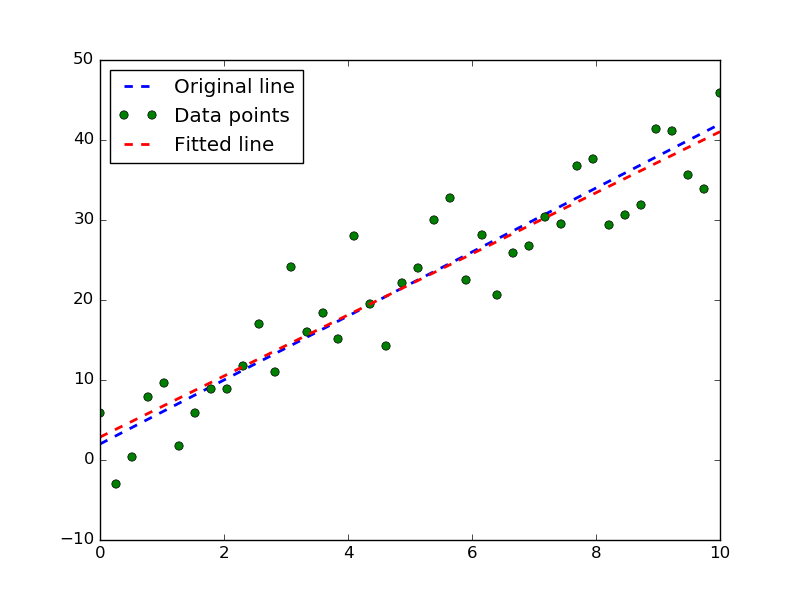
\includegraphics[width=\linewidth]{images/line_fit.png}
    \caption{Line of best fit found using parametric mininimization}
\end{figure}
\newpage

\noindent An example of extending $fit\_line$ to higher-degree polynomials can be found in the appendix.

\section{Portfolio Optimization}
\noindent Now that wee have the tools to optimize a function, we can use it to optimize our portfolio! We can choose to optimize/minimize/maximize various measures, such as daily returns, cumulative returns, or Sharpe Ratio based on the percent allocation of all of the stocks in the portfolio.

\subsection{Framing the problem}
\noindent First we need three things:
\begin{enumerate}
\item a function, $f(x)$, to minimize
\item an initial guess for $x$
\item the optimizer
\end{enumerate}

\noindent In our case, $x$ is actually the set of allocations for the stocks. Also, since we want to maximize Sharpe Ratio, we need to multiply $f(x)$ by -1 to call the minimizer.